\documentclass[12pt, letterpaper, twoside]{book}
\raggedbottom
\usepackage{graphicx}
\graphicspath{ {images/} }
\usepackage[utf8]{inputenc}
\usepackage{fullpage}
\usepackage[paperheight=11in,paperwidth=8.5in,margin=0in]{geometry}
\usepackage{amsmath}
\usepackage{listings}
\date{4nd June 2021}
\begin{document}
\begin{titlepage}
	\begin{center}
       \vspace*{5cm}
       \bfseries\Large
    	Assignment 5\\
    	Of\\
    	Modelling \& Simulation Lab (CS1052)\\
        \vskip1cm
        Masters of Technology in Computer Science And Engineering\\
        \vskip1cm
        submitted by\\
    	Arghya Bandyopadhyay\\
    	RollNo. 20CS4103\\
    	\vskip1cm
    	submitted to\\
    	Dr Nanda Dulal Jana\\
    	Assistant Professor\\
    	Dept. of CSE\\
    	\vskip1cm
    	
\includegraphics[width=4cm]{NITDGP}\\
    	National Institute of Technology, Durgapur\\
    \end{center}
\end{titlepage}
\begin{center}
\textbf{\\Problem 1}
\end{center}
\begin{flushleft}
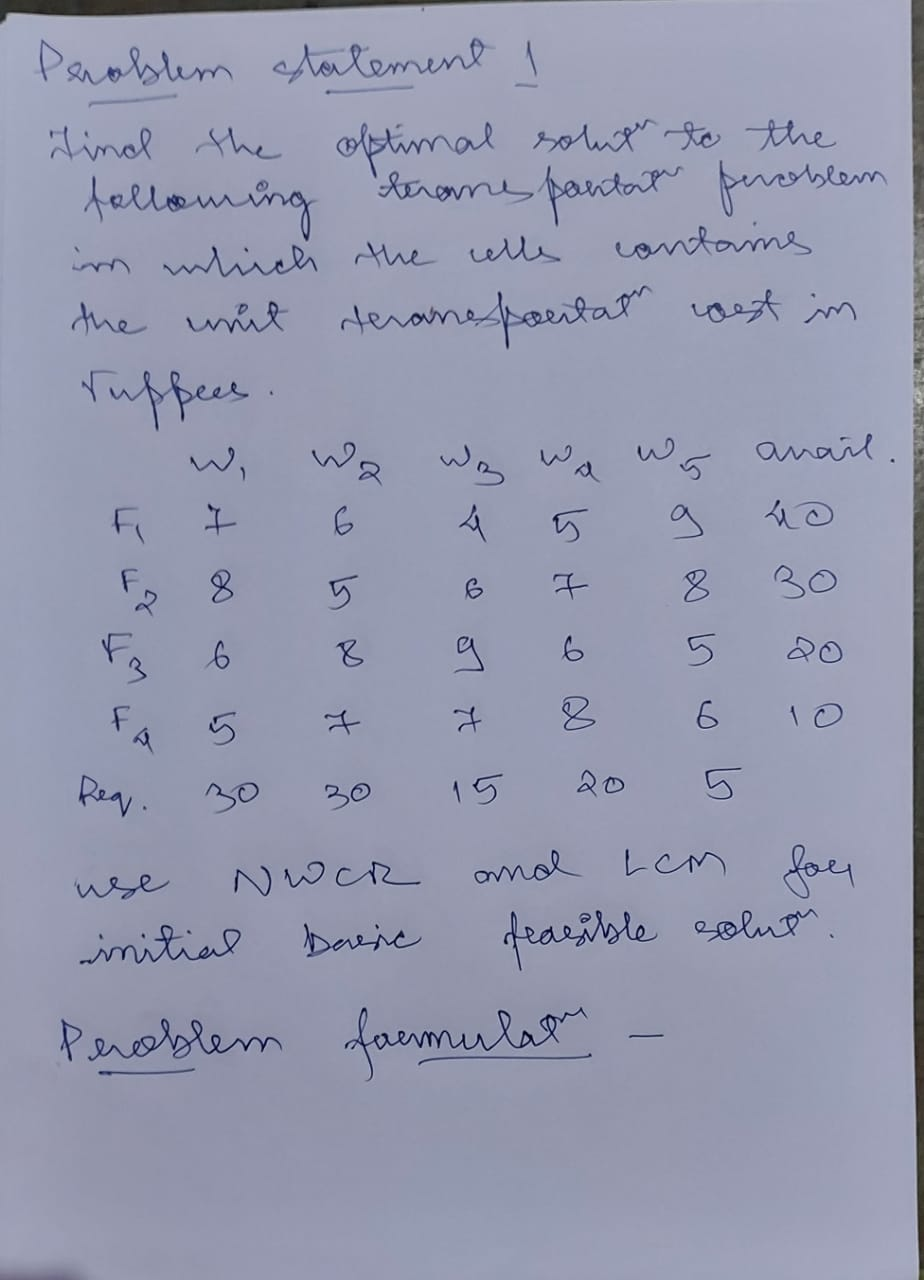
\includegraphics[width=\paperwidth, height=10in]{Page1}
\end{flushleft}
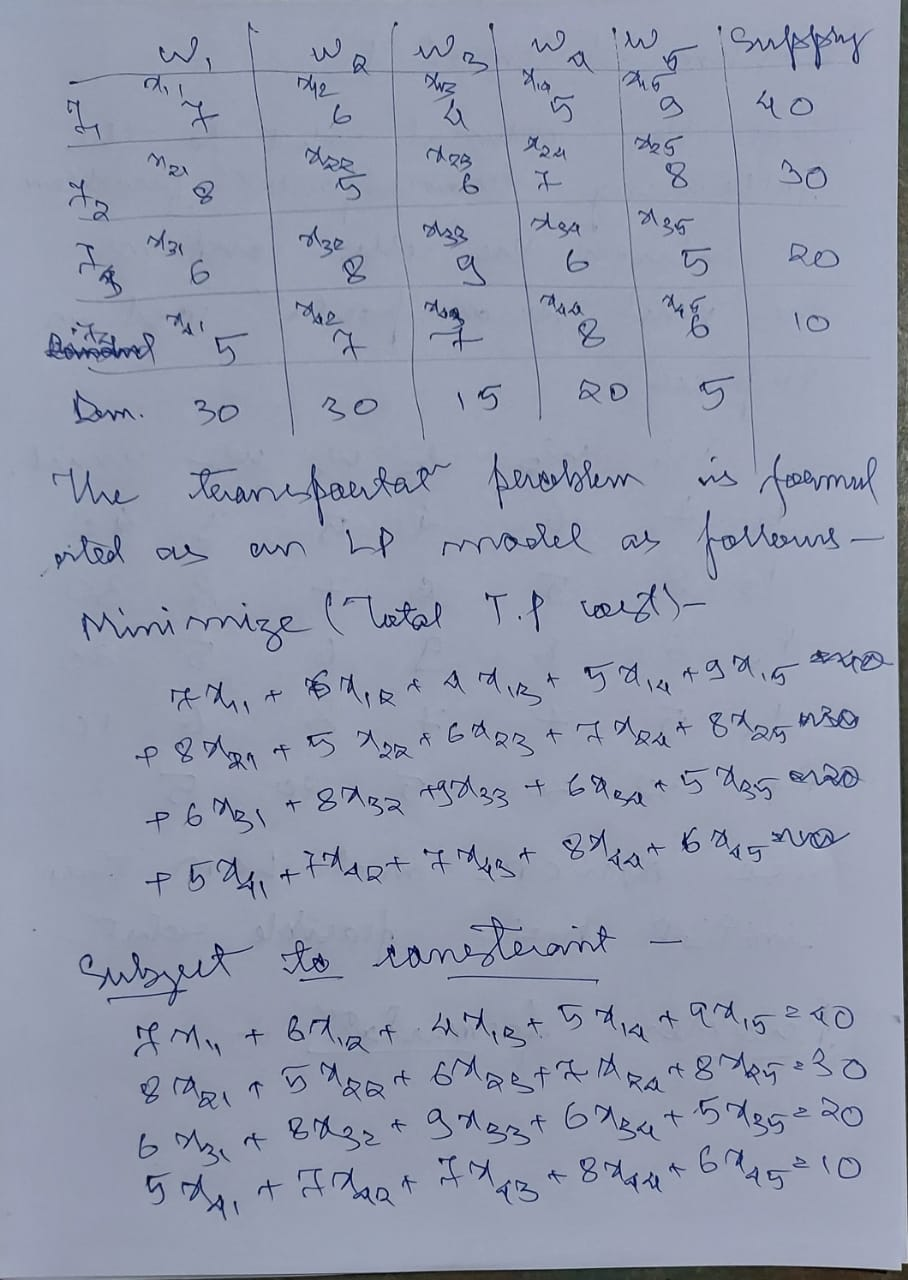
\includegraphics[width=\paperwidth, height=\paperheight]{Page2}
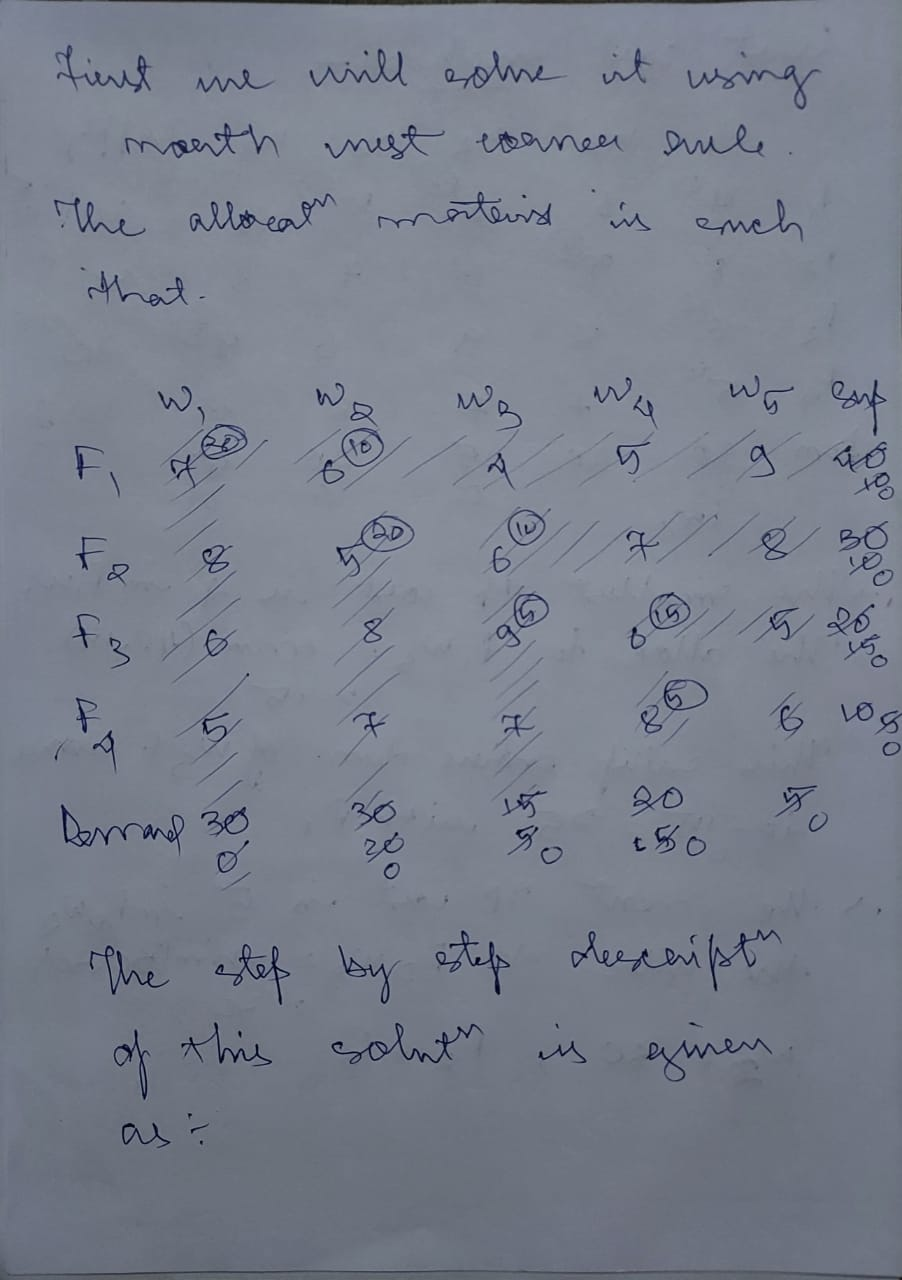
\includegraphics[width=\paperwidth, height=\paperheight]{Page3}
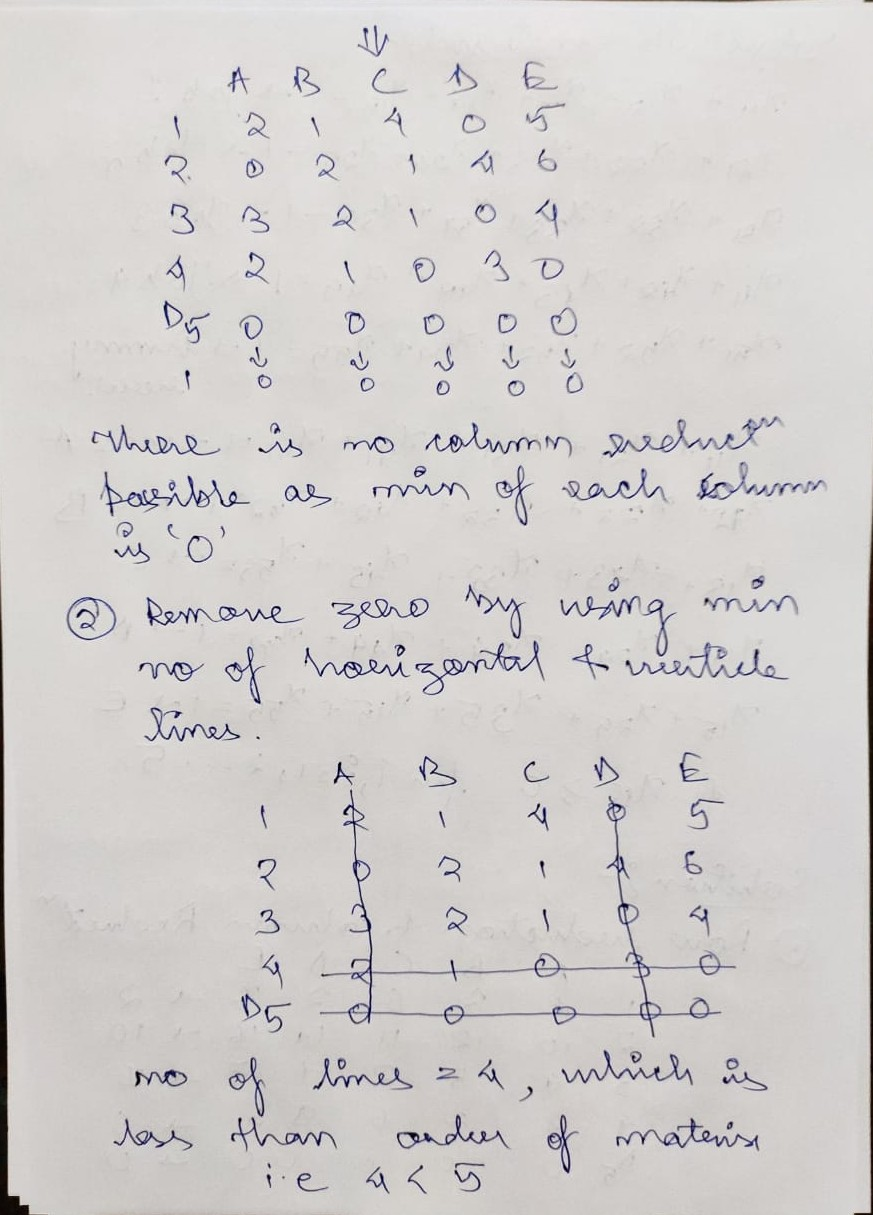
\includegraphics[width=\paperwidth, height=\paperheight]{Page4}
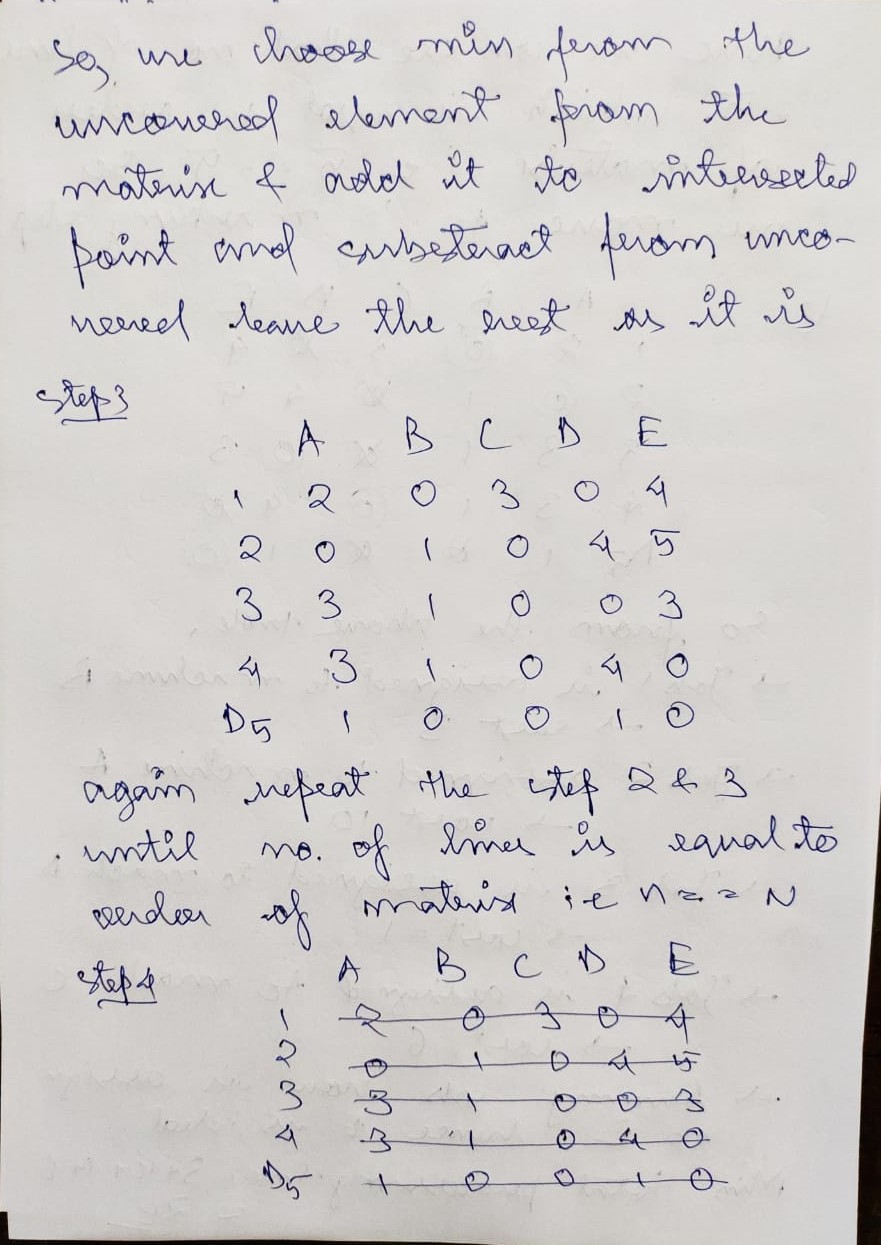
\includegraphics[width=\paperwidth, height=\paperheight]{Page5}
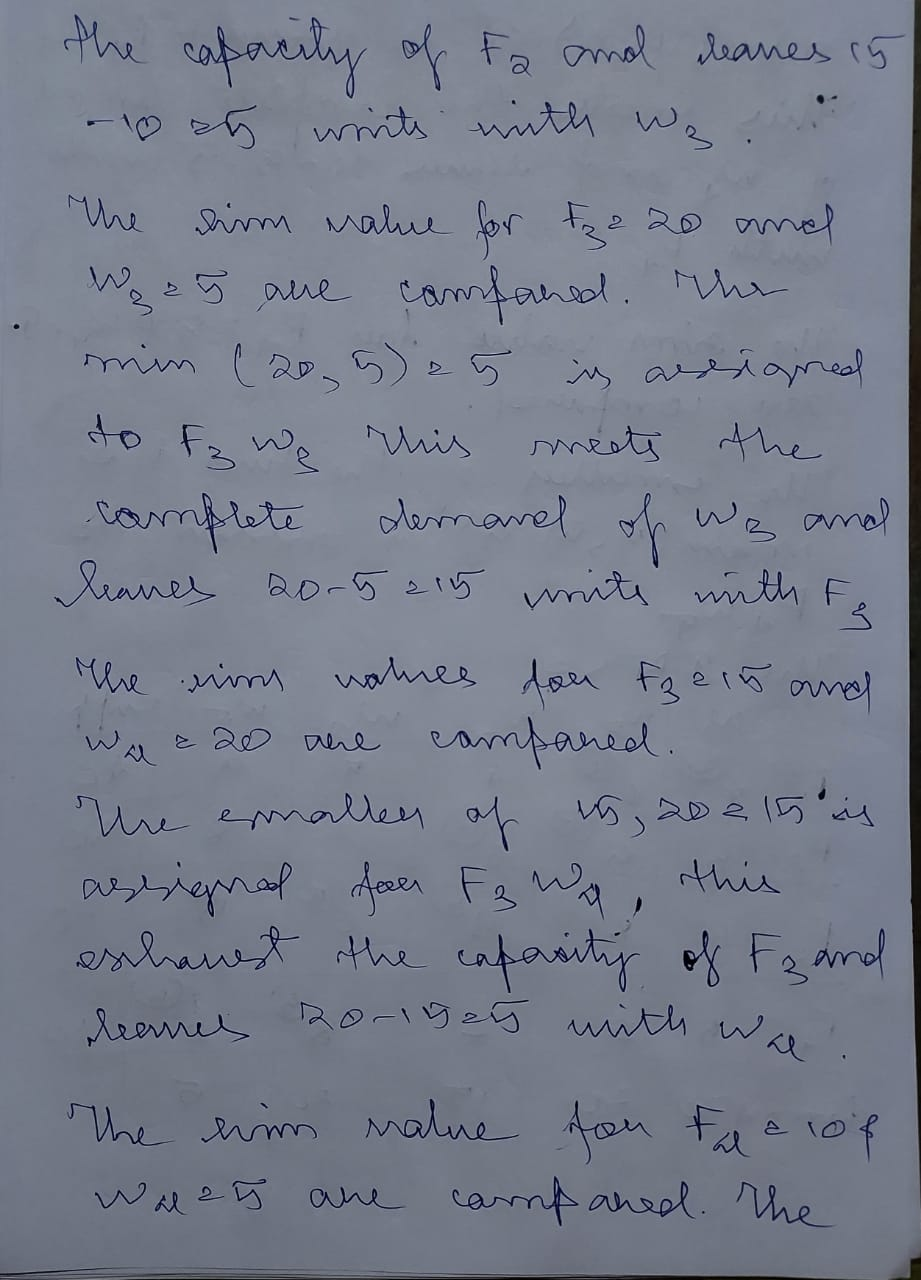
\includegraphics[width=\paperwidth, height=\paperheight]{Page6}

\begin{lstlisting}

Python Code:
	
class HungarianError(Exception):
pass

try:
    import numpy as np
except ImportError:
    raise HungarianError("NumPy is not installed.")


class Hungarian:
    """
    Implementation of the Hungarian (Munkres) Algorithm using np.
    Usage:
        hungarian = Hungarian(cost_matrix)
        hungarian.calculate()
    or
        hungarian = Hungarian()
        hungarian.calculate(cost_matrix)
    Handle Profit matrix:
        hungarian = Hungarian(profit_matrix, is_profit_matrix=True)
    or
        cost_matrix = Hungarian.make_cost_matrix(profit_matrix)
    The matrix will be automatically padded if it is not square.
    For that numpy's resize function is used, which automatically adds 0's to any row/column that is added
    Get results and total potential after calculation:
        hungarian.get_results()
        hungarian.get_total_potential()
    """

    def __init__(self, input_matrix=None, is_profit_matrix=False):
        """
        input_matrix is a List of Lists.
        input_matrix is assumed to be a cost matrix unless is_profit_matrix is True.
        """
        if input_matrix is not None:
            # Save input
            my_matrix = np.array(input_matrix)
            self._input_matrix = np.array(input_matrix)
            self._maxColumn = my_matrix.shape[1]
            self._maxRow = my_matrix.shape[0]

            # Adds 0s if any columns/rows are added. Otherwise stays unaltered
            matrix_size = max(self._maxColumn, self._maxRow)
            pad_columns = matrix_size - self._maxRow
            pad_rows = matrix_size - self._maxColumn
            my_matrix = np.pad(my_matrix, ((0, pad_columns), (0, pad_rows)), 'constant', constant_values=(0))

            # Convert matrix to profit matrix if necessary
            if is_profit_matrix:
                my_matrix = self.make_cost_matrix(my_matrix)

            self._cost_matrix = my_matrix
            self._size = len(my_matrix)
            self._shape = my_matrix.shape

            # Results from algorithm.
            self._results = []
            self._totalPotential = 0
        else:
            self._cost_matrix = None

    def get_results(self):
        """Get results after calculation."""
        return self._results

    def get_total_potential(self):
        """Returns expected value after calculation."""
        return self._totalPotential

    def calculate(self, input_matrix=None, is_profit_matrix=False):
        """
        Implementation of the Hungarian (Munkres) Algorithm.
        input_matrix is a List of Lists.
        input_matrix is assumed to be a cost matrix unless is_profit_matrix is True.
        """
        # Handle invalid and new matrix inputs.
        if input_matrix is None and self._cost_matrix is None:
            raise HungarianError("Invalid input")
        elif input_matrix is not None:
            self.__init__(input_matrix, is_profit_matrix)

        result_matrix = self._cost_matrix.copy()

        # Step 1: Subtract row mins from each row.
        for index, row in enumerate(result_matrix):
            result_matrix[index] -= row.min()

        # Step 2: Subtract column mins from each column.
        for index, column in enumerate(result_matrix.T):
            result_matrix[:, index] -= column.min()

        # Step 3: Use minimum number of lines to cover all zeros in the matrix.
        # If the total covered rows+columns is not equal to the matrix size then adjust matrix and repeat.
        total_covered = 0
        while total_covered < self._size:
            # Find minimum number of lines to cover all zeros in the matrix and find total covered rows and columns.
            cover_zeros = CoverZeros(result_matrix)
            covered_rows = cover_zeros.get_covered_rows()
            covered_columns = cover_zeros.get_covered_columns()
            total_covered = len(covered_rows) + len(covered_columns)

            # if the total covered rows+columns is not equal to the matrix size then adjust it by min uncovered num (m).
            if total_covered < self._size:
                result_matrix = self._adjust_matrix_by_min_uncovered_num(result_matrix, covered_rows, covered_columns)

        # Step 4: Starting with the top row, work your way downwards as you make assignments.
        # Find single zeros in rows or columns.
        # Add them to final result and remove them and their associated row/column from the matrix.
        expected_results = min(self._maxColumn, self._maxRow)
        zero_locations = (result_matrix == 0)
        while len(self._results) != expected_results:

            # If number of zeros in the matrix is zero before finding all the results then an error has occurred.
            if not zero_locations.any():
                raise HungarianError("Unable to find results. Algorithm has failed.")

            # Find results and mark rows and columns for deletion
            matched_rows, matched_columns = self.__find_matches(zero_locations)

            # Make arbitrary selection
            total_matched = len(matched_rows) + len(matched_columns)
            if total_matched == 0:
                matched_rows, matched_columns = self.select_arbitrary_match(zero_locations)

            # Delete rows and columns
            for row in matched_rows:
                zero_locations[row] = False
            for column in matched_columns:
                zero_locations[:, column] = False

            # Save Results
            self.__set_results(zip(matched_rows, matched_columns))

        # Calculate total potential
        value = 0
        for row, column in self._results:
            value += self._input_matrix[row, column]
        self._totalPotential = value

    @staticmethod
    def make_cost_matrix(profit_matrix):
        """
        Converts a profit matrix into a cost matrix.
        Expects NumPy objects as input.
        """
        # subtract profit matrix from a matrix made of the max value of the profit matrix
        matrix_shape = profit_matrix.shape
        offset_matrix = np.ones(matrix_shape, dtype=int) * profit_matrix.max()
        cost_matrix = offset_matrix - profit_matrix
        return cost_matrix

    def _adjust_matrix_by_min_uncovered_num(self, result_matrix, covered_rows, covered_columns):
        """Subtract m from every uncovered number and add m to every element covered with two lines."""
        # Calculate minimum uncovered number (m)
        elements = []
        for row_index, row in enumerate(result_matrix):
            if row_index not in covered_rows:
                for index, element in enumerate(row):
                    if index not in covered_columns:
                        elements.append(element)
        min_uncovered_num = min(elements)

        # Add m to every covered element
        adjusted_matrix = result_matrix
        for row in covered_rows:
            adjusted_matrix[row] += min_uncovered_num
        for column in covered_columns:
            adjusted_matrix[:, column] += min_uncovered_num

        # Subtract m from every element
        m_matrix = np.ones(self._shape, dtype=int) * min_uncovered_num
        adjusted_matrix -= m_matrix

        return adjusted_matrix

    def __find_matches(self, zero_locations):
        """Returns rows and columns with matches in them."""
        marked_rows = np.array([], dtype=int)
        marked_columns = np.array([], dtype=int)

        # Mark rows and columns with matches
        # Iterate over rows
        for index, row in enumerate(zero_locations):
            row_index = np.array([index])
            if np.sum(row) == 1:
                column_index, = np.where(row)
                marked_rows, marked_columns = self.__mark_rows_and_columns(marked_rows, marked_columns, row_index,
                                                                           column_index)

        # Iterate over columns
        for index, column in enumerate(zero_locations.T):
            column_index = np.array([index])
            if np.sum(column) == 1:
                row_index, = np.where(column)
                marked_rows, marked_columns = self.__mark_rows_and_columns(marked_rows, marked_columns, row_index,
                                                                           column_index)

        return marked_rows, marked_columns

    @staticmethod
    def __mark_rows_and_columns(marked_rows, marked_columns, row_index, column_index):
        """Check if column or row is marked. If not marked then mark it."""
        new_marked_rows = marked_rows
        new_marked_columns = marked_columns
        if not (marked_rows == row_index).any() and not (marked_columns == column_index).any():
            new_marked_rows = np.insert(marked_rows, len(marked_rows), row_index)
            new_marked_columns = np.insert(marked_columns, len(marked_columns), column_index)
        return new_marked_rows, new_marked_columns

    @staticmethod
    def select_arbitrary_match(zero_locations):
        """Selects row column combination with minimum number of zeros in it."""
        # Count number of zeros in row and column combinations
        rows, columns = np.where(zero_locations)
        zero_count = []
        for index, row in enumerate(rows):
            total_zeros = np.sum(zero_locations[row]) + np.sum(zero_locations[:, columns[index]])
            zero_count.append(total_zeros)

        # Get the row column combination with the minimum number of zeros.
        indices = zero_count.index(min(zero_count))
        row = np.array([rows[indices]])
        column = np.array([columns[indices]])

        return row, column

    def __set_results(self, result_lists):
        """Set results during calculation."""
        # Check if results values are out of bound from input matrix (because of matrix being padded).
        # Add results to results list.
        for result in result_lists:
            row, column = result
            if row < self._maxRow and column < self._maxColumn:
                new_result = (int(row), int(column))
                self._results.append(new_result)


class CoverZeros:
    """
    Use minimum number of lines to cover all zeros in the matrix.
    Algorithm based on: http://weber.ucsd.edu/~vcrawfor/hungar.pdf
    """

    def __init__(self, matrix):
        """
        Input a matrix and save it as a boolean matrix to designate zero locations.
        Run calculation procedure to generate results.
        """
        # Find zeros in matrix
        self._zero_locations = (matrix == 0)
        self._shape = matrix.shape

        # Choices starts without any choices made.
        self._choices = np.zeros(self._shape, dtype=bool)

        self._marked_rows = []
        self._marked_columns = []

        # marks rows and columns
        self.__calculate()

        # Draw lines through all unmarked rows and all marked columns.
        self._covered_rows = list(set(range(self._shape[0])) - set(self._marked_rows))
        self._covered_columns = self._marked_columns

    def get_covered_rows(self):
        """Return list of covered rows."""
        return self._covered_rows

    def get_covered_columns(self):
        """Return list of covered columns."""
        return self._covered_columns

    def __calculate(self):
        """
        Calculates minimum number of lines necessary to cover all zeros in a matrix.
        Algorithm based on: http://weber.ucsd.edu/~vcrawfor/hungar.pdf
        """
        while True:
            # Erase all marks.
            self._marked_rows = []
            self._marked_columns = []

            # Mark all rows in which no choice has been made.
            for index, row in enumerate(self._choices):
                if not row.any():
                    self._marked_rows.append(index)

            # If no marked rows then finish.
            if not self._marked_rows:
                return True

            # Mark all columns not already marked which have zeros in marked rows.
            num_marked_columns = self.__mark_new_columns_with_zeros_in_marked_rows()

            # If no new marked columns then finish.
            if num_marked_columns == 0:
                return True

            # While there is some choice in every marked column.
            while self.__choice_in_all_marked_columns():
                # Some Choice in every marked column.

                # Mark all rows not already marked which have choices in marked columns.
                num_marked_rows = self.__mark_new_rows_with_choices_in_marked_columns()

                # If no new marks then Finish.
                if num_marked_rows == 0:
                    return True

                # Mark all columns not already marked which have zeros in marked rows.
                num_marked_columns = self.__mark_new_columns_with_zeros_in_marked_rows()

                # If no new marked columns then finish.
                if num_marked_columns == 0:
                    return True

            # No choice in one or more marked columns.
            # Find a marked column that does not have a choice.
            choice_column_index = self.__find_marked_column_without_choice()

            while choice_column_index is not None:
                # Find a zero in the column indexed that does not have a row with a choice.
                choice_row_index = self.__find_row_without_choice(choice_column_index)

                # Check if an available row was found.
                new_choice_column_index = None
                if choice_row_index is None:
                    # Find a good row to accomodate swap. Find its column pair.
                    choice_row_index, new_choice_column_index = self.__find_best_choice_row_and_new_column(
                        choice_column_index)

                    # Delete old choice.
                    self._choices[choice_row_index, new_choice_column_index] = False

                # Set zero to choice.
                self._choices[choice_row_index, choice_column_index] = True

                # Loop again if choice is added to a row with a choice already in it.
                choice_column_index = new_choice_column_index

    def __mark_new_columns_with_zeros_in_marked_rows(self):
        """Mark all columns not already marked which have zeros in marked rows."""
        num_marked_columns = 0
        for index, column in enumerate(self._zero_locations.T):
            if index not in self._marked_columns:
                if column.any():
                    row_indices, = np.where(column)
                    zeros_in_marked_rows = (set(self._marked_rows) & set(row_indices)) != set([])
                    if zeros_in_marked_rows:
                        self._marked_columns.append(index)
                        num_marked_columns += 1
        return num_marked_columns

    def __mark_new_rows_with_choices_in_marked_columns(self):
        """Mark all rows not already marked which have choices in marked columns."""
        num_marked_rows = 0
        for index, row in enumerate(self._choices):
            if index not in self._marked_rows:
                if row.any():
                    column_index, = np.where(row)
                    if column_index in self._marked_columns:
                        self._marked_rows.append(index)
                        num_marked_rows += 1
        return num_marked_rows

    def __choice_in_all_marked_columns(self):
        """Return Boolean True if there is a choice in all marked columns. Returns boolean False otherwise."""
        for column_index in self._marked_columns:
            if not self._choices[:, column_index].any():
                return False
        return True

    def __find_marked_column_without_choice(self):
        """Find a marked column that does not have a choice."""
        for column_index in self._marked_columns:
            if not self._choices[:, column_index].any():
                return column_index

        raise HungarianError(
            "Could not find a column without a choice. Failed to cover matrix zeros. Algorithm has failed.")

    def __find_row_without_choice(self, choice_column_index):
        """Find a row without a choice in it for the column indexed. If a row does not exist then return None."""
        row_indices, = np.where(self._zero_locations[:, choice_column_index])
        for row_index in row_indices:
            if not self._choices[row_index].any():
                return row_index

        # All rows have choices. Return None.
        return None

    def __find_best_choice_row_and_new_column(self, choice_column_index):
        """
        Find a row index to use for the choice so that the column that needs to be changed is optimal.
        Return a random row and column if unable to find an optimal selection.
        """
        row_indices, = np.where(self._zero_locations[:, choice_column_index])
        for row_index in row_indices:
            column_indices, = np.where(self._choices[row_index])
            column_index = column_indices[0]
            if self.__find_row_without_choice(column_index) is not None:
                return row_index, column_index

        # Cannot find optimal row and column. Return a random row and column.
        from random import shuffle

        shuffle(row_indices)
        column_index, = np.where(self._choices[row_indices[0]])
        return row_indices[0], column_index[0]

\end{lstlisting}
\pagebreak
\begin{lstlisting}

if __name__ == '__main__':

    cost_matrix = [
        [4, 3, 6, 2, 7],
        [10, 12, 11, 14, 16],
        [4, 3, 2, 1, 5],
        [8, 7, 6, 9, 6]]

    hungarian = Hungarian(cost_matrix)
    hungarian.calculate()
    print("Cost Matrix : \n", np.array(cost_matrix))
    jobs = [1, 2, 3, 4]
    machine = ['A', 'B', 'C', 'D', 'E']
    result = hungarian.get_results()
    print("Job-Machine Assignment:")
    for i in result:
        print("Job-", jobs[i[0]], "-> Machine -", machine[i[1]], " is having Cost =", cost_matrix[i[0]][i[1]])
    print("Total Processing Time:\t", hungarian.get_total_potential())
    print("-" * 80)

\end{lstlisting}
\pagebreak
\begin{lstlisting}

	Output:

\end{lstlisting}


\includegraphics[width=550pt]{Output1}
\pagebreak

\begin{center}
\textbf{\\Problem 2}
\end{center}
\begin{flushleft}
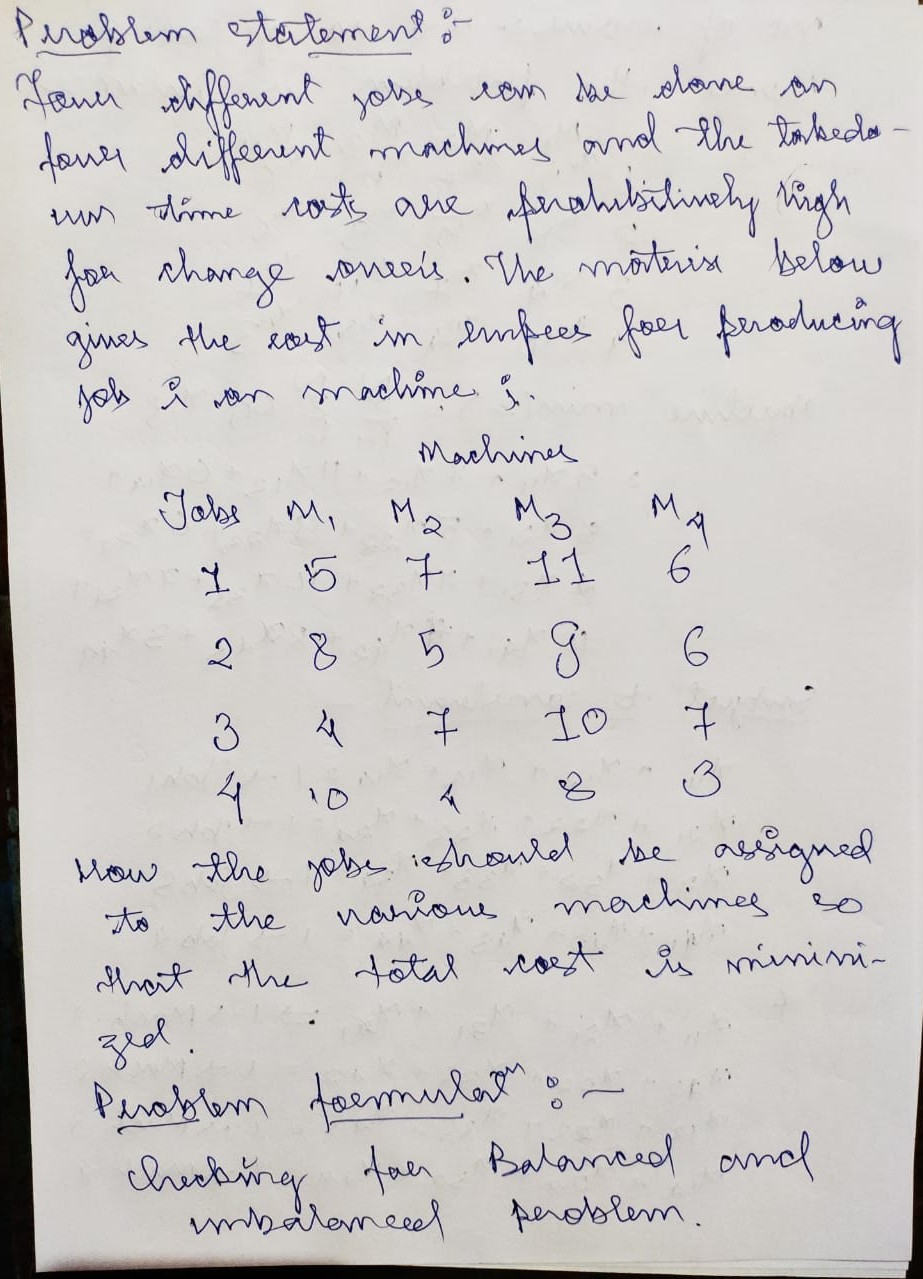
\includegraphics[width=\paperwidth, height=10in]{Page7}
\end{flushleft}
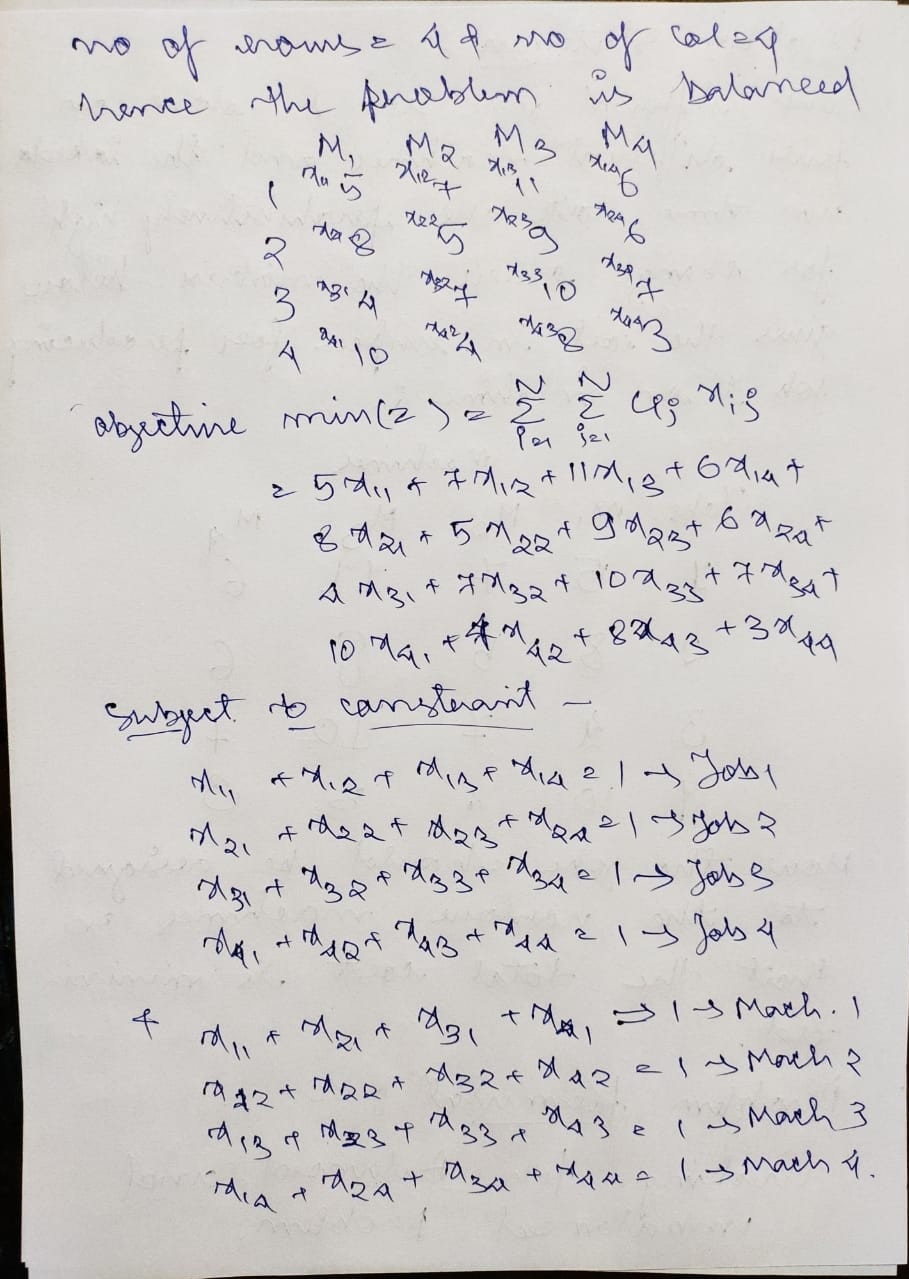
\includegraphics[width=\paperwidth, height=\paperheight]{Page8}
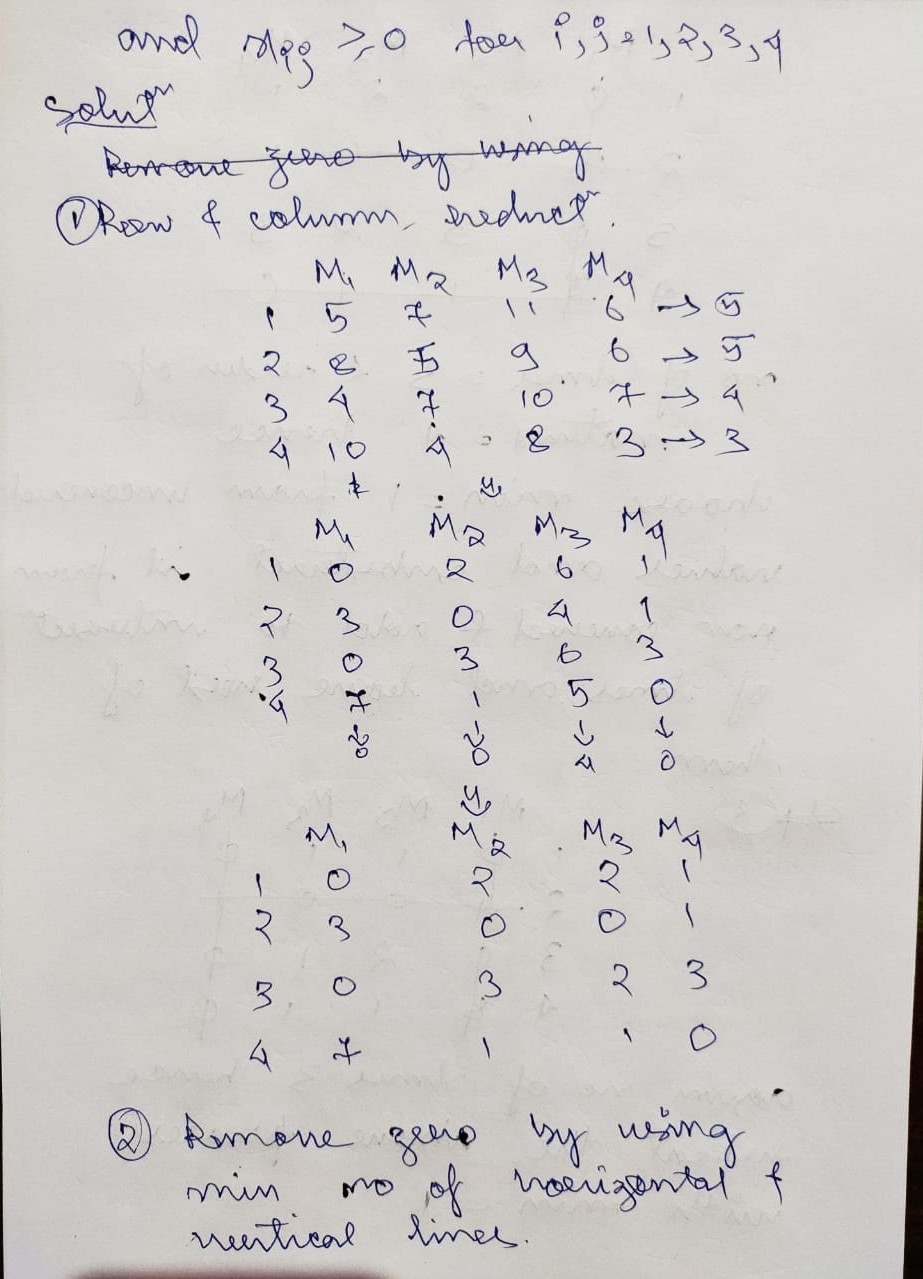
\includegraphics[width=\paperwidth, height=\paperheight]{Page9}
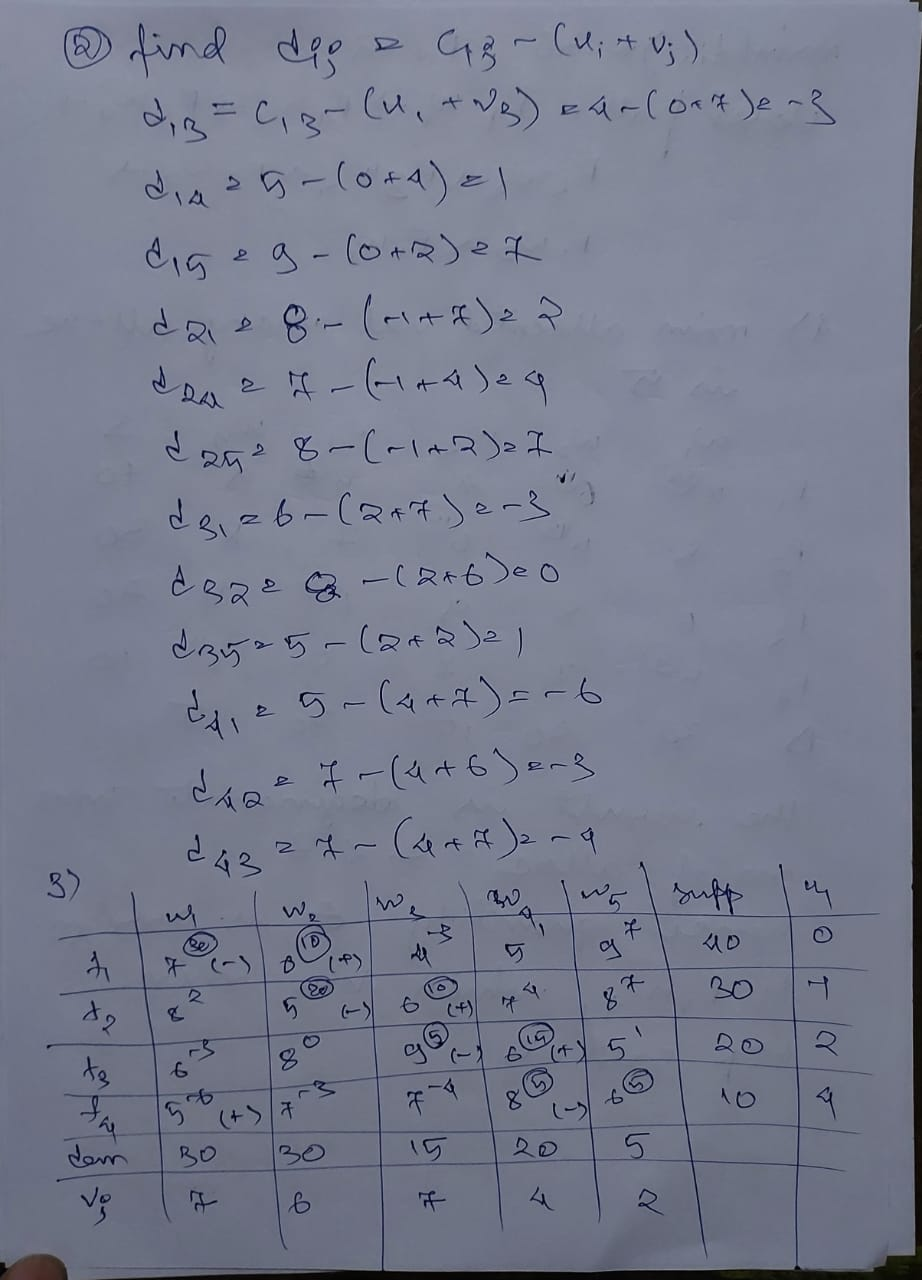
\includegraphics[width=\paperwidth, height=\paperheight]{Page10}
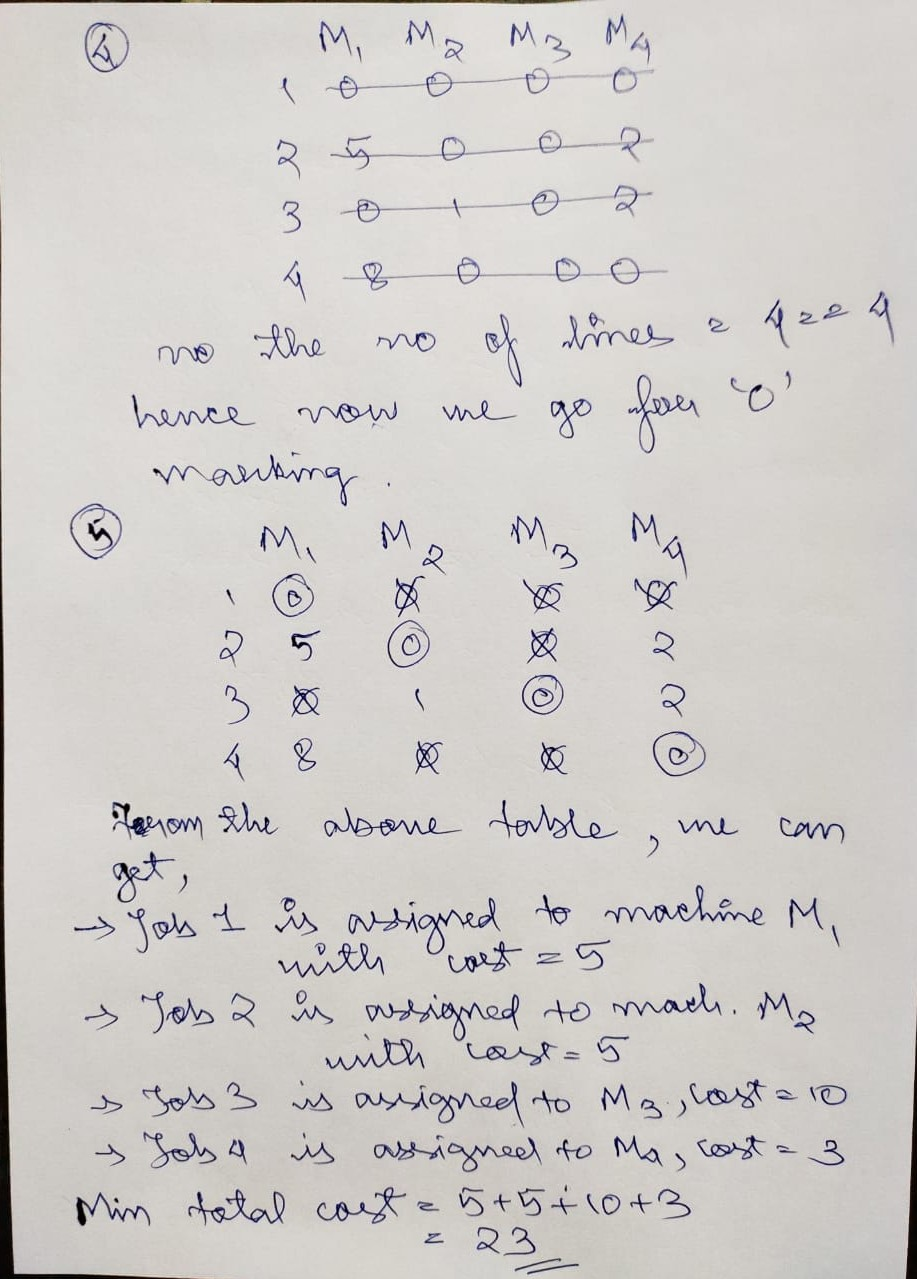
\includegraphics[width=\paperwidth, height=\paperheight]{Page11}
\begin{lstlisting}    
	
Python Code:
	
class HungarianError(Exception):
pass

try:
    import numpy as np
except ImportError:
    raise HungarianError("NumPy is not installed.")


class Hungarian:
    """
    Implementation of the Hungarian (Munkres) Algorithm using np.
    Usage:
        hungarian = Hungarian(cost_matrix)
        hungarian.calculate()
    or
        hungarian = Hungarian()
        hungarian.calculate(cost_matrix)
    Handle Profit matrix:
        hungarian = Hungarian(profit_matrix, is_profit_matrix=True)
    or
        cost_matrix = Hungarian.make_cost_matrix(profit_matrix)
    The matrix will be automatically padded if it is not square.
    For that numpy's resize function is used, which automatically adds 0's to any row/column that is added
    Get results and total potential after calculation:
        hungarian.get_results()
        hungarian.get_total_potential()
    """

    def __init__(self, input_matrix=None, is_profit_matrix=False):
        """
        input_matrix is a List of Lists.
        input_matrix is assumed to be a cost matrix unless is_profit_matrix is True.
        """
        if input_matrix is not None:
            # Save input
            my_matrix = np.array(input_matrix)
            self._input_matrix = np.array(input_matrix)
            self._maxColumn = my_matrix.shape[1]
            self._maxRow = my_matrix.shape[0]

            # Adds 0s if any columns/rows are added. Otherwise stays unaltered
            matrix_size = max(self._maxColumn, self._maxRow)
            pad_columns = matrix_size - self._maxRow
            pad_rows = matrix_size - self._maxColumn
            my_matrix = np.pad(my_matrix, ((0, pad_columns), (0, pad_rows)), 'constant', constant_values=(0))

            # Convert matrix to profit matrix if necessary
            if is_profit_matrix:
                my_matrix = self.make_cost_matrix(my_matrix)

            self._cost_matrix = my_matrix
            self._size = len(my_matrix)
            self._shape = my_matrix.shape

            # Results from algorithm.
            self._results = []
            self._totalPotential = 0
        else:
            self._cost_matrix = None

    def get_results(self):
        """Get results after calculation."""
        return self._results

    def get_total_potential(self):
        """Returns expected value after calculation."""
        return self._totalPotential

    def calculate(self, input_matrix=None, is_profit_matrix=False):
        """
        Implementation of the Hungarian (Munkres) Algorithm.
        input_matrix is a List of Lists.
        input_matrix is assumed to be a cost matrix unless is_profit_matrix is True.
        """
        # Handle invalid and new matrix inputs.
        if input_matrix is None and self._cost_matrix is None:
            raise HungarianError("Invalid input")
        elif input_matrix is not None:
            self.__init__(input_matrix, is_profit_matrix)

        result_matrix = self._cost_matrix.copy()

        # Step 1: Subtract row mins from each row.
        for index, row in enumerate(result_matrix):
            result_matrix[index] -= row.min()

        # Step 2: Subtract column mins from each column.
        for index, column in enumerate(result_matrix.T):
            result_matrix[:, index] -= column.min()

        # Step 3: Use minimum number of lines to cover all zeros in the matrix.
        # If the total covered rows+columns is not equal to the matrix size then adjust matrix and repeat.
        total_covered = 0
        while total_covered < self._size:
            # Find minimum number of lines to cover all zeros in the matrix and find total covered rows and columns.
            cover_zeros = CoverZeros(result_matrix)
            covered_rows = cover_zeros.get_covered_rows()
            covered_columns = cover_zeros.get_covered_columns()
            total_covered = len(covered_rows) + len(covered_columns)

            # if the total covered rows+columns is not equal to the matrix size then adjust it by min uncovered num (m).
            if total_covered < self._size:
                result_matrix = self._adjust_matrix_by_min_uncovered_num(result_matrix, covered_rows, covered_columns)

        # Step 4: Starting with the top row, work your way downwards as you make assignments.
        # Find single zeros in rows or columns.
        # Add them to final result and remove them and their associated row/column from the matrix.
        expected_results = min(self._maxColumn, self._maxRow)
        zero_locations = (result_matrix == 0)
        while len(self._results) != expected_results:

            # If number of zeros in the matrix is zero before finding all the results then an error has occurred.
            if not zero_locations.any():
                raise HungarianError("Unable to find results. Algorithm has failed.")

            # Find results and mark rows and columns for deletion
            matched_rows, matched_columns = self.__find_matches(zero_locations)

            # Make arbitrary selection
            total_matched = len(matched_rows) + len(matched_columns)
            if total_matched == 0:
                matched_rows, matched_columns = self.select_arbitrary_match(zero_locations)

            # Delete rows and columns
            for row in matched_rows:
                zero_locations[row] = False
            for column in matched_columns:
                zero_locations[:, column] = False

            # Save Results
            self.__set_results(zip(matched_rows, matched_columns))

        # Calculate total potential
        value = 0
        for row, column in self._results:
            value += self._input_matrix[row, column]
        self._totalPotential = value

    @staticmethod
    def make_cost_matrix(profit_matrix):
        """
        Converts a profit matrix into a cost matrix.
        Expects NumPy objects as input.
        """
        # subtract profit matrix from a matrix made of the max value of the profit matrix
        matrix_shape = profit_matrix.shape
        offset_matrix = np.ones(matrix_shape, dtype=int) * profit_matrix.max()
        cost_matrix = offset_matrix - profit_matrix
        return cost_matrix

    def _adjust_matrix_by_min_uncovered_num(self, result_matrix, covered_rows, covered_columns):
        """Subtract m from every uncovered number and add m to every element covered with two lines."""
        # Calculate minimum uncovered number (m)
        elements = []
        for row_index, row in enumerate(result_matrix):
            if row_index not in covered_rows:
                for index, element in enumerate(row):
                    if index not in covered_columns:
                        elements.append(element)
        min_uncovered_num = min(elements)

        # Add m to every covered element
        adjusted_matrix = result_matrix
        for row in covered_rows:
            adjusted_matrix[row] += min_uncovered_num
        for column in covered_columns:
            adjusted_matrix[:, column] += min_uncovered_num

        # Subtract m from every element
        m_matrix = np.ones(self._shape, dtype=int) * min_uncovered_num
        adjusted_matrix -= m_matrix

        return adjusted_matrix

    def __find_matches(self, zero_locations):
        """Returns rows and columns with matches in them."""
        marked_rows = np.array([], dtype=int)
        marked_columns = np.array([], dtype=int)

        # Mark rows and columns with matches
        # Iterate over rows
        for index, row in enumerate(zero_locations):
            row_index = np.array([index])
            if np.sum(row) == 1:
                column_index, = np.where(row)
                marked_rows, marked_columns = self.__mark_rows_and_columns(marked_rows, marked_columns, row_index,
                                                                           column_index)

        # Iterate over columns
        for index, column in enumerate(zero_locations.T):
            column_index = np.array([index])
            if np.sum(column) == 1:
                row_index, = np.where(column)
                marked_rows, marked_columns = self.__mark_rows_and_columns(marked_rows, marked_columns, row_index,
                                                                           column_index)

        return marked_rows, marked_columns

    @staticmethod
    def __mark_rows_and_columns(marked_rows, marked_columns, row_index, column_index):
        """Check if column or row is marked. If not marked then mark it."""
        new_marked_rows = marked_rows
        new_marked_columns = marked_columns
        if not (marked_rows == row_index).any() and not (marked_columns == column_index).any():
            new_marked_rows = np.insert(marked_rows, len(marked_rows), row_index)
            new_marked_columns = np.insert(marked_columns, len(marked_columns), column_index)
        return new_marked_rows, new_marked_columns

    @staticmethod
    def select_arbitrary_match(zero_locations):
        """Selects row column combination with minimum number of zeros in it."""
        # Count number of zeros in row and column combinations
        rows, columns = np.where(zero_locations)
        zero_count = []
        for index, row in enumerate(rows):
            total_zeros = np.sum(zero_locations[row]) + np.sum(zero_locations[:, columns[index]])
            zero_count.append(total_zeros)

        # Get the row column combination with the minimum number of zeros.
        indices = zero_count.index(min(zero_count))
        row = np.array([rows[indices]])
        column = np.array([columns[indices]])

        return row, column

    def __set_results(self, result_lists):
        """Set results during calculation."""
        # Check if results values are out of bound from input matrix (because of matrix being padded).
        # Add results to results list.
        for result in result_lists:
            row, column = result
            if row < self._maxRow and column < self._maxColumn:
                new_result = (int(row), int(column))
                self._results.append(new_result)


class CoverZeros:
    """
    Use minimum number of lines to cover all zeros in the matrix.
    Algorithm based on: http://weber.ucsd.edu/~vcrawfor/hungar.pdf
    """

    def __init__(self, matrix):
        """
        Input a matrix and save it as a boolean matrix to designate zero locations.
        Run calculation procedure to generate results.
        """
        # Find zeros in matrix
        self._zero_locations = (matrix == 0)
        self._shape = matrix.shape

        # Choices starts without any choices made.
        self._choices = np.zeros(self._shape, dtype=bool)

        self._marked_rows = []
        self._marked_columns = []

        # marks rows and columns
        self.__calculate()

        # Draw lines through all unmarked rows and all marked columns.
        self._covered_rows = list(set(range(self._shape[0])) - set(self._marked_rows))
        self._covered_columns = self._marked_columns

    def get_covered_rows(self):
        """Return list of covered rows."""
        return self._covered_rows

    def get_covered_columns(self):
        """Return list of covered columns."""
        return self._covered_columns

    def __calculate(self):
        """
        Calculates minimum number of lines necessary to cover all zeros in a matrix.
        Algorithm based on: http://weber.ucsd.edu/~vcrawfor/hungar.pdf
        """
        while True:
            # Erase all marks.
            self._marked_rows = []
            self._marked_columns = []

            # Mark all rows in which no choice has been made.
            for index, row in enumerate(self._choices):
                if not row.any():
                    self._marked_rows.append(index)

            # If no marked rows then finish.
            if not self._marked_rows:
                return True

            # Mark all columns not already marked which have zeros in marked rows.
            num_marked_columns = self.__mark_new_columns_with_zeros_in_marked_rows()

            # If no new marked columns then finish.
            if num_marked_columns == 0:
                return True

            # While there is some choice in every marked column.
            while self.__choice_in_all_marked_columns():
                # Some Choice in every marked column.

                # Mark all rows not already marked which have choices in marked columns.
                num_marked_rows = self.__mark_new_rows_with_choices_in_marked_columns()

                # If no new marks then Finish.
                if num_marked_rows == 0:
                    return True

                # Mark all columns not already marked which have zeros in marked rows.
                num_marked_columns = self.__mark_new_columns_with_zeros_in_marked_rows()

                # If no new marked columns then finish.
                if num_marked_columns == 0:
                    return True

            # No choice in one or more marked columns.
            # Find a marked column that does not have a choice.
            choice_column_index = self.__find_marked_column_without_choice()

            while choice_column_index is not None:
                # Find a zero in the column indexed that does not have a row with a choice.
                choice_row_index = self.__find_row_without_choice(choice_column_index)

                # Check if an available row was found.
                new_choice_column_index = None
                if choice_row_index is None:
                    # Find a good row to accomodate swap. Find its column pair.
                    choice_row_index, new_choice_column_index = self.__find_best_choice_row_and_new_column(
                        choice_column_index)

                    # Delete old choice.
                    self._choices[choice_row_index, new_choice_column_index] = False

                # Set zero to choice.
                self._choices[choice_row_index, choice_column_index] = True

                # Loop again if choice is added to a row with a choice already in it.
                choice_column_index = new_choice_column_index

    def __mark_new_columns_with_zeros_in_marked_rows(self):
        """Mark all columns not already marked which have zeros in marked rows."""
        num_marked_columns = 0
        for index, column in enumerate(self._zero_locations.T):
            if index not in self._marked_columns:
                if column.any():
                    row_indices, = np.where(column)
                    zeros_in_marked_rows = (set(self._marked_rows) & set(row_indices)) != set([])
                    if zeros_in_marked_rows:
                        self._marked_columns.append(index)
                        num_marked_columns += 1
        return num_marked_columns

    def __mark_new_rows_with_choices_in_marked_columns(self):
        """Mark all rows not already marked which have choices in marked columns."""
        num_marked_rows = 0
        for index, row in enumerate(self._choices):
            if index not in self._marked_rows:
                if row.any():
                    column_index, = np.where(row)
                    if column_index in self._marked_columns:
                        self._marked_rows.append(index)
                        num_marked_rows += 1
        return num_marked_rows

    def __choice_in_all_marked_columns(self):
        """Return Boolean True if there is a choice in all marked columns. Returns boolean False otherwise."""
        for column_index in self._marked_columns:
            if not self._choices[:, column_index].any():
                return False
        return True

    def __find_marked_column_without_choice(self):
        """Find a marked column that does not have a choice."""
        for column_index in self._marked_columns:
            if not self._choices[:, column_index].any():
                return column_index

        raise HungarianError(
            "Could not find a column without a choice. Failed to cover matrix zeros. Algorithm has failed.")

    def __find_row_without_choice(self, choice_column_index):
        """Find a row without a choice in it for the column indexed. If a row does not exist then return None."""
        row_indices, = np.where(self._zero_locations[:, choice_column_index])
        for row_index in row_indices:
            if not self._choices[row_index].any():
                return row_index

        # All rows have choices. Return None.
        return None

    def __find_best_choice_row_and_new_column(self, choice_column_index):
        """
        Find a row index to use for the choice so that the column that needs to be changed is optimal.
        Return a random row and column if unable to find an optimal selection.
        """
        row_indices, = np.where(self._zero_locations[:, choice_column_index])
        for row_index in row_indices:
            column_indices, = np.where(self._choices[row_index])
            column_index = column_indices[0]
            if self.__find_row_without_choice(column_index) is not None:
                return row_index, column_index

        # Cannot find optimal row and column. Return a random row and column.
        from random import shuffle

        shuffle(row_indices)
        column_index, = np.where(self._choices[row_indices[0]])
        return row_indices[0], column_index[0]

\end{lstlisting}
\pagebreak
\begin{lstlisting}

if __name__ == '__main__':
    cost_matrix = [
        [5, 7, 11, 6],
        [8, 5, 9, 6],
        [4, 7, 10, 7],
        [10, 4, 8, 3]]

    hungarian = Hungarian(cost_matrix)
    hungarian.calculate()
    print("Cost Matrix : \n", np.array(cost_matrix))
    jobs = [1, 2, 3, 4]
    machine = ['M1', 'M2', 'M3', 'M4']
    result = hungarian.get_results()
    print("Job-Machine Assignment:")
    for i in result:
        print("Job-", jobs[i[0]], "-> Machine -", machine[i[1]], " is having Cost =", cost_matrix[i[0]][i[1]])
    print("Total Processing Time:\t", hungarian.get_total_potential())
    print("-" * 80)

\end{lstlisting}
\pagebreak
\begin{lstlisting}

	Output:

\end{lstlisting}

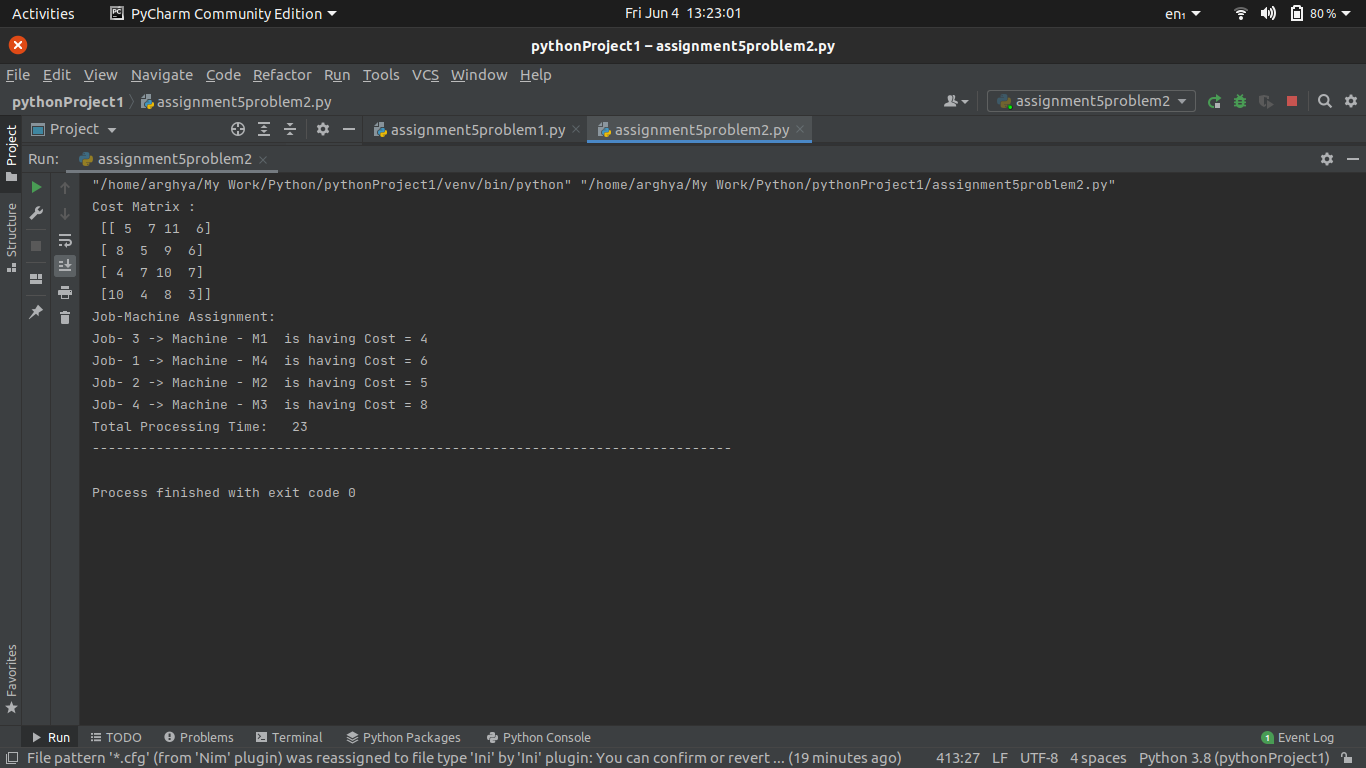
\includegraphics[width=550pt]{Output2}

\end{document}
